%%%%%%%%%%%%%%%%%%%%%%%%%%%%%%%%%%%%%%%%%%%%%%%
%%%%%%%%%%%%%%%%%%%%%%%%%%%%%%%%%%%%%%%%%%%%%%%
\setcounter{section}{1}\section{国際的なSKA計画の歩み}
\label{c01.s2}

%%%%%%%%%%%%%%%%%%%%%%%%%%%%%%%%%%%%%%%%%%%%%%%
%%%%%%%%%%%%%%%%%%%%%%%%%%%%%%%%%%%%%%%%%%%%%%%
\subsection{組織}
\label{c01.s2.ss1}

\paragraph{参加国}

2015年1月現在、オーストラリア・南アフリカ・ニュージーランド・イギリス・イタリア・オランダ・中国・カナダ・ドイツ・ノルウェー・インドの11ヶ国が、各国政府の予算支援の下でSKAメンバー国となっている。SKA計画の最終意思決定を行うBoard会議はこのSKAメンバー国で構成される。SKA1の予算確保が始まっており、英国が1億ポンドの予算を計上したのを皮切りに、イタリアでも予算交渉が進んでいる。一方で、ドイツは2014年度をもって主要参加国から脱退する見込みとなっているが、予算の負担割合は3 \%弱のため計画への予算的影響は限定的である。以上のメンバー国以外にも参加を目指す国が複数あり、例えばフランスやポルトガルが準備段階に入っている。日本はアメリカなどと同様に、まだ大型予算を割いて計画に参加する段階にはない。しかし関心を持つ国として、個人や研究機関レベルの協力が進んでいる。

\paragraph{SKA機構}

SKA1の建設前段階に入る2013年前後に、SKAの本部機能は大幅に増強された。現在、SKA計画はその増強されたSKA機構(SKA OrganizationまたはSKA Office、SKAO)が運営している。SKAOは英国ジョドレルバンク観測所内に本部を構え、2014年11月時点で46名の専属スタッフと4名の長期滞在者・契約職員が在籍している。組織の構成は次のとおりである。

\begin{itemize}
\item[★] 機構長Philip Diamond

\begin{itemize}

\item[●] 副機構長・プロジェクト長Alistair McPherson
\begin{itemize}
\item[◆] 設計部門 責任者Tim Cornwell、副責任者Peter Dewdney
\begin{itemize}
\item[-] ドメインスペシャリスト集団(工学系の設計・監督)
\end{itemize}
\item[◆] システムエンジニアリング(SE)部門 責任者Tim Stevenson
\begin{itemize}
\item[-] SEメンバー集団(工学系の設計・検査)
\end{itemize}
\item[◆] プロジェクトマネージャー集団(各コンソーシアムの連絡・調査・管理)
\item[◆] プロジェクト調整スタッフ(計画調整・構成)
\end{itemize}

\item[●] 科学部門 責任者Robert Braun
\begin{itemize}
\item[-] 科学部門メンバー(理学系の設計・監督)
\end{itemize}

\item[●] 政策部門 責任者Simon Berry
\begin{itemize}
\item[-] 政策スタッフ(ポリシー・産業界連携など)
\end{itemize}

\item[●] 管理部門 責任者Colin Greenwood
\begin{itemize}
\item[-] 管理スタッフ(総務・財務・ITなど)
\end{itemize}

\item[●] 広報部門 責任者William Garnier
\begin{itemize}
\item[-] 広報スタッフ(ウェブ・月刊誌など)
\end{itemize}

\end{itemize}
\end{itemize}
なお2018年に建設期へ移行する際に、SKAOは本部の移転を行う予定である。その本部がSKA計画の恒久的な本部となる。イギリスとイタリアがその候補地に立候補しており、2015年3月のSKA Board会議にて候補地が決定される予定である。

\paragraph{Science Working Groups (SWG)とFocus groups (FG)}

SKA計画の科学検討は、世界各国の研究者が参加するScience Working Groups (SWG)
\begin{itemize}
\item[◆] 宇宙再電離(Epoch of Reionization)
\item[◆] 連続波(Continuum)
\item[◆] 宇宙論(Cosmology)
\item[◆] 宇宙生命(Cradle of Life)
\item[◆] HI銀河(HI galaxy science)
\item[◆] 宇宙磁場(Magnetism)
\item[◆] パルサー(Pulsars)
\item[◆] 突発天体(Transients)
\end{itemize}
とFocus groups (FG)
\begin{itemize}
\item[◆] 銀河系(Our Galaxy)
\item[◆] スペクトル線(Spectral Line)
\item[◆] 超長基線干渉計(VLBI)
\end{itemize}
が行っている。SWGは代表、コアメンバー、そして連携メンバーからなる。科学的見地から設計の問題点を指摘したり、後述の国際SKAサイエンスブックの執筆を行ってきた。SKAOの各担当はその活動の支援を行っている。

\paragraph{Work Package Consortia (WPC)}

SKA計画の設計と開発を支えるのは、世界各国のさまざまな研究機関・民間団体が参加するWork Package Consortia (WPC)である。WPCは
\begin{itemize}
\item[◆] パラボナアンテナ(Dish、DSH)
\item[◆] 低周波開口アンテナ(Low Frequency Aperture Array、LFAA)
\item[◆] 中周波開口アンテナ(Mid Frequency Aperture Array、MFAA)
\item[◆] 広帯域フィード(Wide Band Single Pixel Feed、WBSPF)
\item[◆] 信号データ転送(Signal and Data Transport、SaDT)
\item[◆] 中央信号処理(Central Signal Processor、CSP)
\item[◆] 科学データ処理(Science Data Prosessor、SDP)
\item[◆] 望遠鏡管理(Telescope Management、TM)
\item[◆] 組み立てならびに検査(Assembly, Integration, and Verification、AIV)
\item[◆] 南アフリカ公共設備(Infrastructure in South Africa、INFRA SA)
\item[◆] オーストラリア公共設備(Infrastructure in Australia、 INFRA AU)
\end{itemize}
に分かれている。WPCは要素ないしサブシステムレベルでのアイデアやオプションをSKAOに提案し、また各種の検査を引き受けている。SKAOの各担当はその活動の支援を行っている。


%%%%%%%%%%%%%%%%%%%%%%%%%%%%%%%%%%%%%%%%%%%%%%%
%%%%%%%%%%%%%%%%%%%%%%%%%%%%%%%%%%%%%%%%%%%%%%%
\subsection{建設地}
\label{c01.s2.ss2}

\paragraph{建設地の決定} 

2012年3月に干渉計建設地が決定した。南アフリカとその周辺国、オーストラリアとニュージーランド、の2団体が候補地に名乗りを上げていたが、結果的に両地域に分散して建設することに決まった。

\paragraph{アフリカの計画} 

南アフリカとその周辺国の計画は次のとおりである。SKA1では190台の直径15 m SKAパラボナアンテナと64台の直径13.5 m MeerKATパラボナアンテナを用いる(SKA1-MID)。 これらはSingle Pixel Feed (SPF)を搭載する。SKA2ではSKAパラボナアンテナをおよそ10倍の2,000台に増やし、最大3,000 kmにまで分布させる(SKA2-MID)。そしてPhased Array Feed (PAF)という広視野観測を可能にする最新装置、または広帯域フィード(WBSPF)を搭載する。また250の中間波長高密集開口アンテナ局を設置し、広視野観測をする(SKA2-MFAA)。

\paragraph{オセアニアの計画} 

オーストラリアとニュージーランドの計画は次のとおりである。SKA1では25万台の長波長開口アンテナを900局程度に分散して設置する(SKA1-LOW)。また60台の直径15m SKAパラボナアンテナと36台の直径12m ASKAPパラボナアンテナを用いる(SKA1-SUR)。これにはPAFを搭載する。SKA2では長波長開口アンテナだけを残し、アンテナ数をおよそ4倍の100万台にまで増やす(SKA2-LOW)。

%%%%%%%%%%%%%%%%%%%%%%%%%%%%%%%%%%%%%%%%%%%%%%%
%%%%%%%%%%%%%%%%%%%%%%%%%%%%%%%%%%%%%%%%%%%%%%%
\subsection{スケジュール(SKA1とSKA2)}
\label{c01.s2.ss3}

\paragraph{建設スケジュール} 

SKA1を中心としたスケジュールを図\ref{c01.s2.f1}に示す。2015年1月現在は、SKA1の建設前段階の前期(SKA1 Pre-constructuin stage 1)にある。2013年3月にSKA1のBaseline Designが公表されてから2015年2月までの間で、スケジュールはほぼ予定通り消化されている。

\paragraph{Re-Baselining Submissions (RBS)}

2014年に入って、SKA Board会議はSKA1の建設費の上限額を650Mユーロと定めた。同じ頃、結成されたWPCからの提案などにもとづいて、考えられる多くの機能を盛り込んだ場合、その建設費は上限額を大幅に上回ることがわかった。もちろん、全機能を盛り込むというのは全く現実的ではないが、とはいえ様々に提案された選択肢から予算上限に収まる現実的な機能を絞り込む必要があった。そこで当初のスケジュールにはない基本デザインの修正(Re-Baselining Submissions、RBS)が、2014年度に進められた。経費の削減案は、サイエンスへの影響を数値化しながら、サブ要素、要素、システム、実運用の4段階で消去法により絞り込まれた。2014年後半からは暫定科学評価委員(Ad hoc Science Review panel、SRP)が集められ、SKAOが行った削減案のサイエンスへの影響評価やリスクが精査された。また科学技術諮問委員会(Science and Engineering Advisory Committee、SEAC)が招集され、SKAOが行ったRBSの行程は適切であったか、SKAOの検討状況は十分だったか、そしてRBSについての方針が議論された。以上のように、組織的、計画的、そして多角的にRBSの検討が行われた。最終的に、SRPやSEACの意見を踏まえた機構長からの修正案が、科学的・技術的な調査資料と合わせてSKA Boardに提出された。2015年3月のSKA Board会議にて、基本デザインが修正される予定である。

\begin{figure}[tbp]
\begin{center}
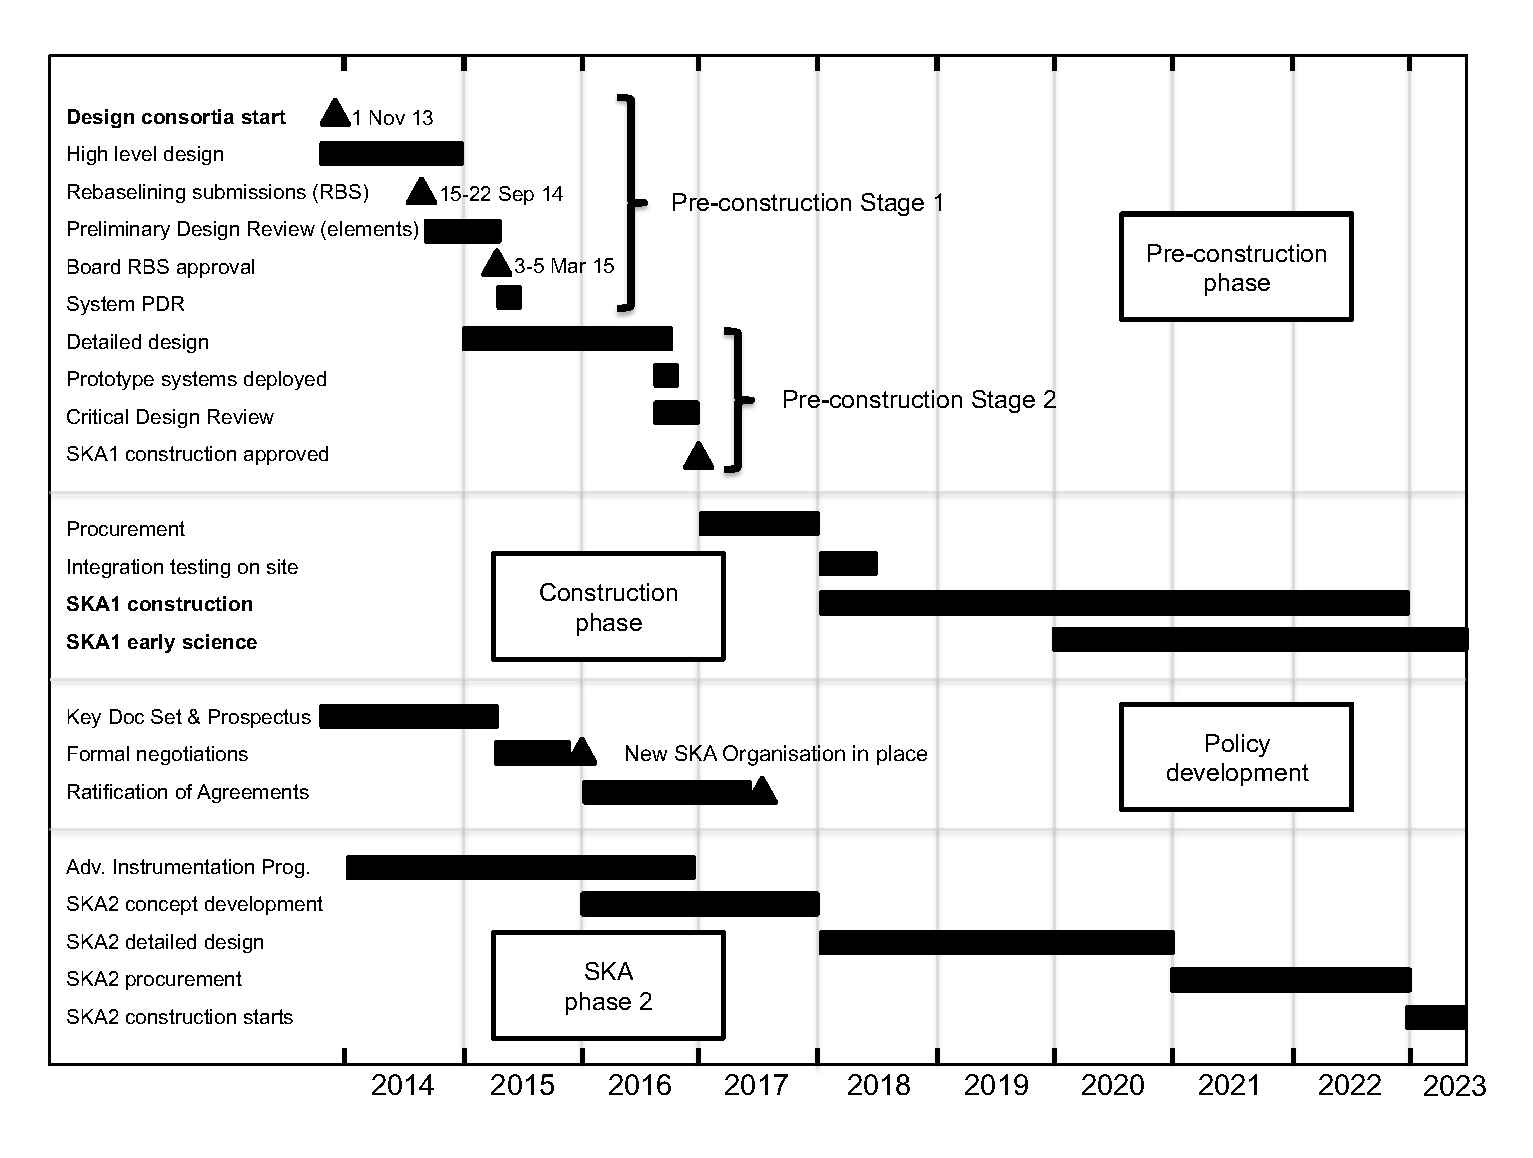
\includegraphics[width=\linewidth]{introduction/c01.s2.f1.eps}
\caption{SKA計画のスケジュール(Alistair McPhersonならびにRobert Braun提供)。}\label{c01.s2.f1}
\end{center}
\end{figure}

\paragraph{国際SKAサイエンスブック2015} 

2004年に出版された国際SKAサイエンスブック2004から10年が経過したことを受けて、2014年度にサイエンスブックの刷新が図られている。そのサイエンスの内容を検討する国際会議が2014年6月にイタリアで開催され、同12月までにはサマリー章を除く論文が採録決定された。すでに多くの論文がarXivに投稿されている。このサイエンスブックの刷新はRBSとは独立しているため、仮に一部の論文が基本デザインの修正と整合しない場合でもそのまま出版される。SKAOはRBSの結果に対するコメントを最終的に載せて、2015年の春に出版をする予定である。本書では、この国際SKAサイエンスブック2015について重点的に触れる。本書で特に断りなく「国際サイエンスブック」と称した場合、この刷新された版を指す。

\paragraph{優先的な科学目標}

前小節ではSKAの主要な科学を紹介したが、デザイン設計やデザイン設計の修正の過程においては、その都度優先的な科学目標が定義されてきた。例えば、2013年3月にSKA1 Baseline Designが設計された際には、宇宙再電離がメートル波の、パルサーがセンチ波の中核的な科学目標と定義づけられた。2014年度のRBSの過程においては、13の具体的な観測プランまで伴った最優先科学目標(Highest Priority Science Objectives、HPSOs)が参照された。
しかし、SRPやSEACの諮問においては、引き続き宇宙再電離とパルサーがSKA1の中核的な科学目標だという認識もあった。


%%%%%%%%%%%%%%%%%%%%%%%%%%%%%%%%%%%%%%%%%%%%%%%
%%%%%%%%%%%%%%%%%%%%%%%%%%%%%%%%%%%%%%%%%%%%%%%
\subsection{今後について}
\label{c01.s2.ss4}

\paragraph{主要科学観測計画} 

SKAはその構想段階においては、SKAメンバー国・非メンバー国の如何を問わず、世界中の研究者が観測に参加でき成果を得ることができるというオープンスカイポリシーを持っていた。しかし、現在はそのポリシーは大幅に変更されている。SKA1においては、観測可能時間の半分以上が長時間の観測プログラムで構成される主要科学計画(Key Science Programs、KSP)に配分される。KSPはSKAメンバー国の研究者でなければ代表を務めることはできない見込みである。そしてKSPから生み出される成果もSKAメンバー国の研究者のものとなる。非メンバー国の研究者が主体となる(例えば論文の筆頭著者になる)のは難しい見通しである。一般公募の観測時間はごくわずかのため、高い競争率が予想される。ゆえにSKAメンバー国とならずとも観測時間が得られると考えるのは早計である。なお、2015年8月にストックホルムにて、このKSPについて意見交換を行う国際会議が開催される。

\paragraph{仮デザイン審査(PDR)を経て詳細設計へ} 

2014年度後半から、SKAOは各コンソーシアムから提案されたシステムや要素レベルでの設計案を順次審査している。この仮デザイン審査(Preliminary Design Review、PDR)後、有望なものがコンソーシアム内で絞り込まれ、詳細設計へと移行される予定である。2015年3月に決定される基本デザインの修正は、程度の差こそあれ仮デザイン審査の追加を必要とするだろう。ただし、基本デザインの修正はすでに存在する要素設計案から経費削減できる修正を絞り込むという方法をとっている。従って要素レベルで全面的な仮デザイン審査のやり直しということは起こらない。スケジュールに与える影響は限定的である。

